\documentclass[a4paper, 11pt, twoside]{report}

% Language and Encoding
\usepackage[utf8]{inputenc}
\usepackage[T1]{fontenc}
\usepackage[italian]{babel}

% Fonts
\usepackage{microtype} % Improves text spacing
\usepackage{fontspec}
\setmainfont[Scale=0.95]{Helvetica}
\setmonofont[Scale=0.9]{IBM Plex Mono}
\newfontfamily\titlefont{Times New Roman}
\usepackage[font=footnotesize]{caption}

% Page Layout & Margins
\usepackage[
    a4paper,
    top=3.0cm,
    bottom=3.0cm,
    inner=2.5cm,
    outer=2.5cm,
    bindingoffset=1cm, % Extra 1cm added purely for the binding side
    headheight=15pt
]{geometry}


% Headers and Footers
\setlength{\headheight}{15pt} % Fix warning about header height
\usepackage{fancyhdr}
\pagestyle{fancy}
\fancyhf{}                    % Clear all defaults
\newif\ifshowlogo
\showlogotrue
\newcommand{\blankpage}{
    \clearpage
    \thispagestyle{empty}     % No headers/footers
    \showlogofalse            % No Logo
    \hbox{}                   % Invisible content
    \newpage
    \showlogotrue             % Resume Logo
}

% Line thickness
\renewcommand{\headrulewidth}{0.4pt}
\renewcommand{\footrulewidth}{0.4pt}
\renewcommand{\chaptermark}[1]{\markboth{#1}{}}

% Style for Chapter pages (plain style usually suppresses headers, we override it)
\fancyhead[LO]{
\includegraphics[height=0.3cm]{header_small_logo.png}}      % Left on Odd
\fancyhead[RO, LE]{\thepage}                                               % Right on Odd
\fancyhead[RE]{\nouppercase{\leftmark}}
\fancyfoot[LO, RE]{\footnotesize \textit{Valutazione di WebGPU per applicazioni di Realtà Virtuale tramite integrazione con OpenXR/OpenVR}}
\renewcommand{\headrulewidth}{0.4pt}
\renewcommand{\footrulewidth}{0.4pt}
\fancypagestyle{plain}{
    \fancyhf{}                                                             % Clear defaults
    \fancyhead[LO]{
\includegraphics[height=0.3cm]{header_small_logo.png}} 
    \fancyhead[RO, LE]{\thepage}
    \fancyhead[RE]{\nouppercase{\leftmark}}
    \fancyfoot[LO, RE]{\footnotesize \textit{Valutazione di WebGPU per applicazioni di Realtà Virtuale tramite integrazione con OpenXR/OpenVR}}
    \renewcommand{\headrulewidth}{0.4pt}
    \renewcommand{\footrulewidth}{0.4pt}
}

% Chapter/Section Titles Styling
\usepackage{titlesec}
\usepackage{color}

% Chapter Format
\titleformat{\chapter}[display]
{\normalfont\huge\bfseries}      % Format
{\chaptertitlename\ \thechapter} % Label (e.g., Capitolo 1)
{20pt}                           % Separation
{\Huge}                          % Title size

% Section Format
\titleformat{\section}
{\normalfont\Large\bfseries}
{\thesection}
{1em}
{}

% Graphics & Tables
\usepackage{graphicx}
\usepackage[most]{tcolorbox}
\usepackage{booktabs}
\usepackage{array}

% Code Snippets
\usepackage{minted}
\usepackage{xcolor}
\usemintedstyle{emacs}
\setminted{
numbersep=5pt,
frame=lines,
framesep=2mm,
fontsize=\small,
}
\renewcommand{\theFancyVerbLine}{
    \textcolor{darkgray}{\tiny\ttfamily\arabic{FancyVerbLine}}
}

% Hyperlinks
\usepackage[hidelinks]{hyperref}

% Absolute Positioning Package
\usepackage{eso-pic}
\AddToShipoutPictureBG{%
   \ifshowlogo
   \ifodd\value{page}%
     \AtPageLowerLeft{%
       \put(\LenToUnit{\dimexpr\paperwidth-1.5cm\relax}, \LenToUnit{2cm}){%
          
\includegraphics[height=5cm, keepaspectratio]{supsistudent_logo.png}%
       }%
     }%
   \else
     \AtPageLowerLeft{%
       \put(\LenToUnit{1.0cm}, \LenToUnit{2cm}){%
          
\includegraphics[height=5cm, keepaspectratio]{supsistudent_logo.png}%
       }%
     }%
   \fi
   \fi
}

\usepackage{listings}
\usepackage{xcolor}
\usepackage{geometry}
\geometry{margin=2.5cm}

% Bibliography
\usepackage{csquotes}
\usepackage[backend=biber, style=numeric, sorting=none]{biblatex}
\addbibresource{bibliography.bib}

% Glossary
\usepackage[toc]{glossaries}
\makeglossaries
\loadglsentries{glossary.tex}

% PDF Metadata
\hypersetup{
    pdftitle={Progetto di Diploma},
    pdfauthor={Mazza Luca},
    pdfsubject={Valutazione di WebGPU per applicazioni di Realtà Virtuale tramite integrazione con OpenXR/OpenVR},
    pdfkeywords={WebGPU, OpenXR, OpenVR, C++, VR, AR, XR},
    pdfproducer={XeLaTeX},
    pdfcreator={XeLaTeX with hyperref}
}

\newenvironment{dedication}
{%\clearpage
  \thispagestyle{empty}
  \vspace*{\stretch{2}}
  \itshape
  \raggedright
}
{\par
 \vspace{\stretch{3}}
 \clearpage
}

\begin{document}

% Custom Title Page 
\begin{titlepage}
\pagenumbering{alph}
\newgeometry{top=2cm, bottom=2cm, left=2.5cm, right=2.5cm}

% Top Header Region
\noindent

\includegraphics[height=2.5cm, keepaspectratio]{header_logo.png}
\hfill

\vspace{0.1cm}

% Title Region
\begin{flushleft}
\titlefont 
    {\Huge Valutazione di WebGPU per applicazioni di Realtà Virtuale tramite integrazione con OpenXR/OpenVR} \\[0.8cm]
\end{flushleft}
\vspace{1cm}

\hrule height 1pt
\vspace{8pt}

\newcommand{\field}[2]{%
    \noindent{\footnotesize #1}\\[8pt] % Label (Small)
    {\Large \textbf{#2}}\par           % Content (Large & Bold)
}

\noindent
\begin{minipage}[t]{0.48\textwidth} 
    \vspace{0pt} % Ensures alignment at the top
    \field{Studente/i}{Mazza Luca}
\end{minipage}%
\hfill
\begin{minipage}[t]{0.48\textwidth}
    \vspace{0pt}
    \field{Relatore}{Peternier Achille}
    \vspace{35pt}\hrule height 1pt\vspace{8pt} % Line separator
    \field{Correlatore}{Paoliello Marco}
    \vspace{35pt}\hrule height 1pt\vspace{8pt} % Line separator
    \field{Committente}{Peternier Achille}
\end{minipage}

\vspace{40pt}

\hrule height 1pt
\vspace{8pt}

\noindent
\begin{minipage}[t]{0.525\textwidth}
    \vspace{0pt}
    \field{Corso di laurea}{Ingegneria informatica \\ (Informatica TP)}
\end{minipage}%
\hfill
\begin{minipage}[t]{0.6\textwidth}
    \vspace{0pt}
    \field{Modulo}{C11287}
\end{minipage}

\vspace{35pt}
\hrule height 1pt % Thicker main divider line
\vspace{8pt}

\noindent
\field{Anno}{2025 / 2026}
\vspace{5cm}                          % Space at the very bottom
\hrule height 1pt width 0.5\textwidth % Thicker main divider line
\vspace{8pt}
\noindent
\begin{minipage}[t]{\textwidth}
    \vspace{0pt}
    \field{Data}{\today}
\end{minipage}
\end{titlepage}
\restoregeometry

\blankpage

\showlogofalse
\begin{dedication}
    Vorrei qui ringraziare
    \textnormal{}\newline
\end{dedication}

\blankpage

% Front Matter
\pagenumbering{roman}
\tableofcontents
\blankpage

% List of Figures/Tables (Optional)
\listoffigures
\blankpage
\listoftables
\blankpage
\renewcommand\listoflistingscaption{Elenco dei codici sorgente}
\listoflistings
\newpage
\blankpage

\pagenumbering{arabic}
\chapter{Abstract}

\vspace{0.5cm}
\noindent\rule{\textwidth}{0.5pt}
\vspace{0.5cm}

\blankpage

\chapter{Introduzione}

Negli ultimi anni, l'evoluzione delle API grafiche ha portato ad un progressivo allontanamento dagli standard
tradizionali, come \texttt{OpenGL}\footnote{\url{https://opengl.org}}, in favore di soluzioni più moderne, che 
forniscono più controllo direttamente sull'hardware delle unità grafiche dei calcolatori.
In questo panorama, \texttt{WebGPU}\footnote{\url{https://webgpu.org}} si è imposta non solo come nuova generazione di
API grafiche per il Web, ma anche come una solida alternativa per contesti nativi, grazie ai kit di sviluppo che la
rendono compatibile con diversi linguaggi a basso livello, come \texttt{C++} e \texttt{Rust}.
Un progetto precedentemente sviluppato ha già analizzato e dimostrato l'efficacia della transizione da \texttt{OpenGL} a
\texttt{WebGPU} per corsi introduttivi alla computer grafica.

Lo scopo del presente progetto è di estendere tale studio di fattibilità in un settore con ancora maggiori esigenze,
ovvero il dominio della \textit{Realtà Virtuale} (VR).
L'obbiettivo principale è la valutazione dell'impiego di \texttt{WebGPU} in un ambiente nativo \texttt{C/C++}, e che
questo possa rappresentare una valida alternativa ad \texttt{OpenGL} per lo sviluppo di applicazioni VR, investigando la
complessità e l'efficacia della sua integrazione con framework standard quali \texttt{\gls{OpenXR}}
\footnote{\url{https://khronos.org/openxr}} e \texttt{\gls{OpenVR}}
\footnote{\url{https://github.com/ValveSoftware/openvr}}.

Come per quanto riguarda i progetti precedentemente sviluppati, per valutare correttamente questa tecnologia è
fondamentale tener sempre presente il contesto accademico in cui si andrà ad operare. Questo lavoro si rivolge in primis
al modulo opzionale \texttt{M-I6331Z - Realtà Virtuale} della SUPSI, che si basa sulle
conoscenze acquisite nel corso obbligatorio \texttt{M-I5203 - Grafica}. Lo scopo di tale corso è di insegnare allo
studente lo sviluppo di un'applicazione interattiva in C++, interfacciandosi direttamente con le API di basso livello,
senza affidarsi a game engine preconfezionati.

In questo scenario, la semplicità d'utilizzo è cruciale nel determinare la fattibilità; una soluzione troppo complessa
rischierebbe di spostare inavvertitamente il focus del corso. Gli studenti e il docente si ritroverebbero a dedicare
troppo tempo a districarsi tra le difficoltà di implementazione dell'API grafica, sottraendolo all'apprendimento
dei concetti fondamentali della Realtà Virtuale. Tuttavia, lo sviluppo VR impone requisiti stringenti in termini di
latenza, prestazioni e gestione diretta dell'hardware, elementi dove le API moderne come \texttt{WebGPU} eccellono,
grazie al loro paradigma basato su pipeline esplicite.

Durante il progetto verrà pertanto sviluppato un prototipo funzionante che utilizzi \texttt{WebGPU} come backend grafico
per il rendering di una scena VR stereoscopica. Verrà creato un layer di integrazione tra WebGPU e le API VR,
affrontando e risolvendo le sfide tecniche legate all'acquisizione delle pose dei dispositivi, alla gestione delle
swapchains e alla rigorosa sincronizzazione dei frame richiesta dal runtime, come ad esempio \texttt{SteamVR}.

L'esito di questa implementazione permetterà infine di confrontare l'approccio \texttt{WebGPU} con le soluzioni
tradizionali, misurando in modo oggettivo il livello di effort richiesto per lo sviluppo e le performance ottenute.
I risultati raccolti forniranno delle linee guida concrete per determinare l'effettiva fattibilità e le
modalità ottimali per l'adozione di \texttt{WebGPU} in ambito didattico e applicativo nel contesto della Realtà
Virtuale.

Con questo documento non si intende però produrre una guida dettagliata per quanto riguarda l'API di \texttt{WebGPU},
e nemmeno all'utilizzo di \texttt{OpenXR} o alle funzionalità VR, bensì saranno espliciti solamente i concetti
essenziali alla comprensione di questo lavoro. Se si desidera apprendere i concetti riguardanti entrambe le API
menzionate si può fare riferimento alla guida per i fondamentali di \texttt{WebGPU}\cite{webgpufundamentals} e a quella
di \texttt{OpenXR}\cite{openxrtutorial}.

È anche da notare che questo documento non ha lo scopo di rendere noto ogni singolo dettaglio di codice sviluppato,
bensì di accompagnare alla comprensione del problema, dei passi intrapresi per cercare di risolverlo e, se finalmente
è fattibile sostituire l'approccio tradizionale con \texttt{WebGPU}.

\section{Pianificazione}

Di seguito sono descritte le differenti fasi atte allo sviluppo del progetto. In quanto la natura del progetto sia
sperimentale, ed infine l'obbiettivo sia quello di verificare la fattibilità di utilizzo, il piano di lavoro non eccede
nei dettagli o nei vincoli ma risulta completo, garantendo la flessibilità necessaria e l'immediata risposta ad
eventuali problemi o deviazioni dai mezzi discussi inizialmente.

\begin{enumerate}
    \item \textbf{Analisi \texttt{WebGPU}}: Analizzare l'approccio necessario per lo sviluppo di un'applicazione grafica
        facente uso dell'API di \texttt{WebGPU}.
    \item \textbf{Analisi \texttt{OpenXR}}: Analizzare l'approccio utilizzato nei progetti precedenti (specialmente per
        quanto riguarda \textit{\texttt{XRBridge}}\footnote{\url{https://github.com/JollyCookie2000/xr-bridge}}) per lo
        sviluppo di un'applicazione grafica che faccia utilizzo di \texttt{OpenXR} per fornire funzionalità per la
        realtà virtuale.
    \item \textbf{Demo \texttt{WebGPU} indipendente}: Derivante dall'analisi riguardante l'API di \texttt{WebGPU},
        sviluppare una demo che possa rappresentare un punto di partenza per lo sviluppo della demo finale. Questa
        deve concentrarsi sulle funzionalità dell'API \texttt{WebGPU}. Questa demo deve rimanere semplice e ridurre la
        complessità di integrazione di ulteriori funzionalità, specialmente quelle riguardanti la realtà virtuale.
    \item \textbf{Demo \texttt{OpenXR} indipendente}: Derivante dall'analisi riguardante \texttt{OpenXR}, sviluppare una
        demo che possa rappresentare un punto di partenza per lo sviluppo della demo finale. Questa deve concentrarsi 
        sulle funzionalità di realtà virtuale. Questa demo deve essere imperativamente concentrata sui requisiti del
        corso di realtà virtuale e concentrarsi ad adattare unicamente ciò che è necessario per il corso.
        Ulteriormente, questa deve essere integrabile nell'ambiente WebGPU, deve quindi avere un approccio modulare,
        il quale permetterà di rimuovere le funzionalità \texttt{OpenGL} e sostituirle con quelle di \texttt{WebGPU}.
    \item \textbf{Swapchain condivisa}: Sviluppare una swapchain, condivisa tra \texttt{WebGPU} e \texttt{OpenXR}, che
        permetta di condividere le texture da mostrare tramite gli occhi dell'headset, tra l'API \texttt{WebGPU} e
        quella di \texttt{OpenXR}. Ciò si riduce nella produzione di una libreria bridge, che utilizzi uno dei "minimi
        comun denominatori\footnote{WebGPU si interfaccia direttamente con l'API di sistema per la rappresentazione
        nativa di immagini grafiche.}" tra le due tecnologie, in questo caso una tra \texttt{\gls{Vulkan}},
        \texttt{\gls{DirectX}} o \texttt{\gls{Metal}}.
    \item \textbf{Sincronizzazione \& Rendering Stereoscopico}: Integrare la sincronizzazione del loop di
        rendering di \texttt{WebGPU} con i tempi dettati da \texttt{OpenXR}.
        Deve essere inoltre modificata la pipeline di \texttt{WebGPU} per renderizzare la scena due volte, basandosi
        sulle matrici di \textit{projection} e \texttt{view} fornite da \texttt{OpenXR} per occhio sinistro e destro.
    \item \textbf{Demo unificata}: Produrre una demo che unisca tutte le funzionalità richieste dal corso di Realtà
        Virtuale, utilizzando l'architettura prodotta nelle fasi precedenti. Questa deve dimostrare in maniera semplice
        e efficace i risultati ottenibili dalla combinazione di \texttt{WebGPU} e \texttt{OpenXR}.
    \item \textbf{Benchmarking}: Misurare il \gls{framerate} e la latenza della demo, utilizzando appropriati strumenti
        di misurazione.
    \item \textbf{Valutazione \textit{effort}}: Confrontare la pipeline prodotta con quelle utilizzate negli anni
        passati del corso; valutare le principali differenze e le difficoltà di comprensione, la verbosità e
        l'osticita di debug.
    \item \textbf{Linee guida conclusive}: Produrre una guida finale che mostri brevemente le conclusioni tratte durante
        lo sviluppo e che guidi l'eventuale integrazione della pipeline nel corso.
\end{enumerate}

Questo rapporto è stato scritto durante tutta la durata del progetto, parallelamente a tutte le fasi descritte sopra.

\section{Requisiti}
\begin{table}[h]
\centering
\caption{Requisiti del progetto}
\begin{tabular}{@{}lp{12cm}l@{}}
\toprule
\textbf{ID}   & \textbf{Descrizione}                                                                    & \textbf{Note}    \\ \midrule
\texttt{R-00} & Deve presentare un backend \texttt{WebGPU}, con \texttt{wgpu\_native}, in \texttt{C++}  & < \texttt{C++20} \\
\texttt{R-01} & Deve presentare l'integrazione di \texttt{OpenXR} per gestire funzionalità VR/XR        & -                \\
\texttt{R-02} & Deve acquisire i dati di tracciamento dell'\gls{HMD}                                    & -                \\
\texttt{R-03} & Deve gestire allocazione texture e submission duale con swapchains                      & -                \\
\texttt{R-04} & Deve gestire la sincronizzazione con il framerate runtime VR                            & -                \\
\texttt{R-05} & Deve presentare una demo completa di scena 3D, che utilizzi \texttt{WebGPU}             & -                \\
\texttt{R-06} & Deve essere compatibile con Windows e Linux                                             & -                \\
\texttt{R-07} & Deve includere analisi complessità, comparata alla soluzione \texttt{OpenGL}            & -                \\
\texttt{R-08} & Deve includere un'analisi della performance (benchmark)                                 & -                \\
\texttt{R-09} & Deve includere un verdetto finale e guida all'utilizzo                                  & -                \\
\bottomrule
\end{tabular}
\end{table}

\chapter{Stato dell'arte}

Negli ultimi dieci anni, l'ecosistema dello sviluppo di applicazioni grafiche interattive ha visto intercorrere una
trasformazione radicale. L'industria si è pian piano allontanata dai paradigmi tradizionali, basati su macchine a stati
globali, per abbracciare interfacce di programmazione dal carattere esplicito, progettate per rispecchiare fedelmente
l'architettura delle GPU multi-core. Ciò ha portato le API, contrariamente al trend seguito dalla maggior parte
dell'ingegneria del software che si muove verso API di alto livello e astrazioni più vicine allo sviluppatore, a
scendere sempre più di livello, avvicinandosi alla programmazione diretta dell'hardware grafico.

Parallelamente, il settore della Realtà Virtuale e Aumentata, comunemente raggruppato sotto il termine \textit{Spatial
computing} o \texttt{XR}, è maturato, passando da prototipi frammentari guidati da singoli vendor a standard aperti e
unificati.
Soprattutto per questo settore, il mercato ha avuto un moderato picco durante il periodo tra il 2020 ed il 2021, il
quale ha poi visto un rapido declino, dovuto a diversi fattori, ma principalmente a scelte e underperformance dei
produttori; specialmente lo spostamento dei settori di ricerca e sviluppo dei maggiori esponenti, come Microsoft e Meta,
nel settore dell'Intelligenza Artificiale, in maniera affrettata (e poco considerata, visti i risultati ad oggi) ha
posto fine all'evoluzione dei prodotti commerciali.
Anche se il rilascio di un nuovo prodotto Apple nel settore, il prezzo imposto dalla casa di Cupertino non ha aiutato
il mercato a rendere la tecnologia attrattiva.

Questo capitolo analizza le tecnologie attualmente impiegate in ambito didattico e industriale, evidenziando la
crescente trasformazione dell'ecosistema grafico, le limitazioni e "l'invecchiamento" degli approcci tradizionali e
la transizione architetturale verso nuovi standard aperti, come \texttt{\gls{OpenXR}} e \texttt{WebGPU}.

\newpage

\section{Standard didattico - \texttt{OpenGL} \& \texttt{OpenVR}}

Nel contesto accademico e della formazione in computer grafica, il corso di Realtà Virtuale ha fatto affidamento
sull'utilizzo di \texttt{OpenGL} per il rendering e \texttt{OpenVR} per l'interfacciamento con gli HMD.

\textbf{\texttt{OpenGL}}\footnote{\url{https://opengl.org}}, introdotto nel 1992, è un'API implicita basata su una
macchina a stati finiti. Il suo successo decennale, specialmente nell'ambito accademico, deriva dalla curva di
apprendimento che risulta relativamente dolce; l'astrazione di alto livello utilizzata dagli sviluppatori risulta
semplice, in quanto nasconde al programmatore la complessa gestione della memoria video, la sincronizzazione dei thread
e la sottomissione dei comandi alla GPU.
Tuttavia, questa astrazione ha un costo architetturale severo: i driver di \texttt{OpenGL} devono eseguire una massiccia
mole di euristiche in background per tradurre le chiamate high level in istruzioni comprensibili per la scheda grafica,
causando un notevole driver overhead e un'imprevedibilità delle prestazioni, soprattutto del frame stuttering, difetti
critici nell'ambito della realtà virtuale, dove la latenza \textit{motion-to-photon} deve rimanere strettamente
inferiore ai 20 millisecondi.

\textbf{\texttt{OpenVR}}\footnote{\url{https://github.com/ValveSoftware/openvr}}, sviluppato da Valve come SDK per la
piattaforma \texttt{SteamVR}, è stata la prima API di successo commerciale a standardizzare l'accesso a device dedicati
alla realtà virtuale \textit{PC-VR}.
Nata in un periodo di forte sperimentazione, questa tecnologia è intrinsecamente legata all'ecosistema di Valve,
soprattutto con i visori di produzione HTC, per i quali le due aziende hanno collaborato nella produzione.
Si basa su un modello nel quale l'hardware sta al centro dell'attenzione; infatti il runtime costringe l'hardware
concorrente a tradurre i propri dati per renderli compatibili con il formato di un HTC
Vive\footnote{\url{https://vive.com}}, per esempio.
Questa soluzione costringerebbe il programmatore a rilasciare una nuova patch ogni volta che un nuovo controller,
visore o elemento periferico per il sistema VR viene rilasciato.
Pur offrendo un'integrazione diretta e robusta con \texttt{OpenGL}, al momento si tratta di una tecnologia legacy,
non più allineata con la traiettoria dell'industria moderna.

\section{Frammentazione - \texttt{Vulkan}, \texttt{DirectX} \& \texttt{Metal}}

Il limite fisiologico di \texttt{OpenGL} ha portato alla nascita di una nuova generazione di API grafiche di basso
livello; il successore naturale è \textbf{\texttt{\gls{Vulkan}}}, sviluppato dallo stesso Khronos Group,
\textbf{\texttt{\gls{DirectX}}}, sviluppato da Microsoft con l'obbiettivo di spingere il Gaming su PC, e 
\textbf{\texttt{\gls{Metal}}}, di produzione Apple, per tutte le piattaforme correntemente sul mercato (iOS, macOS,
tvOS, ecc...). Sebbene queste API garantiscano prestazioni eccezionali eliminando l'overhead dei driver e permettendo il
multithreading nativo, hanno frammentato drasticamente il mercato, rendendo lo sviluppo multipiattaforma un'impresa
titanica.

Vi sono due fattori critici che rendono queste API problematiche per la didattica:
\begin{enumerate}
    \item \gls{Vulkan} richiede un approccio esplicito alla gestione delle risorse. Il developer deve allocare
        manualmente la memoria, gestire i descriptor set, configurare le pipeline memory barrier e orchestrare le code
        di comandi. Realizzare il rendering di un singolo triangolo colorato utilizzando Vulkan richiede la stesura di
        1000-1500 righe di codice, che a confronto delle 50-100 di OpenGL risultano eccessive per un corso di dieci
        settimane. Inoltre, un corso accademico focalizzato sulla realtà virtuale, dove gli argomenti principali
        dovrebbero essere la stereoscopia, l'interazione spaziale e la cinematica, forzare gli studenti ad apprendere
        quest'API significherebbe consumare l'intero semestre solo per inizializzare l'ambiente grafico.
    \item Apple ha ufficialmente deprecato \texttt{OpenGL} sui propri sistemi operativi, per poi rimuovere completamente
        il supporto nativo a tutte quelle tecnologie non-proprietarie che compongono lo standard \textit{de-facto}
        dell'industria. Attualmente infatti, l'unica API grafica nativa supportata dall'hardware \texttt{Apple Silicon}
        e dai sistemi operativi moderni della casa californiana, è \textbf{\texttt{\gls{Metal}}}. Apple ha rifiutato di
        adottare \texttt{Vulkan}, costringendo gli sviluppatori ad affidarsi a complessi layer di traduzione, come
        \textit{\texttt{MoltenVK}}, per ottenere una parvenza di compatibilità.
        Questa tendenza a murare il proprio giardino distrugge il paradigma \textit{Write once, Compile everywhere},
        rendendo impossibile fornire un ambiente di sviluppo nativo e condiviso tra chi sceglie di utilizzare Windows,
        Linux o macOS.
\end{enumerate}

\section{Comparativa - \texttt{OpenVR} \& \texttt{OpenXR}}

La medesima frammentazione vissuta nel mercato delle API si è ripercossa su quello dell'hardware VR. Per risolvere
questo problema, il \textit{Khronos Group}\footnote{\url{https://khronos.org}} ha rilasciato \texttt{OpenXR}, l'attuale
standard industriale open-source per lo spatial computing, adottato universalmente da tutti i principali produttori,
inclusa Valve stessa, che ha attivamente incoraggiato l'abbandono di \texttt{OpenVR}
\footnote{\url{https://windowscentral.com/steamvr-gets-open-source-upgrade-valve-transitions-openxr-api}}.

Le differenze architetturali tra le due API sono profonde e rappresentano una rivoluzione concettuale nel modo in cui
vengono concepite le applicazioni immersive. Di seguito le principali divergenze

\begin{itemize}
    \item \textbf{Gestione Input (Hardware-Centric/Action-Based)}: in \texttt{OpenVR}, il programmatore interroga
        direttamente l'hardware; questo approccio lo obbliga a riscrivere il codice ogni volta che un nuovo visore o una
        nuova periferica viene rilasciata sul mercato. In risposta a questo problema, \texttt{OpenXR} introduce un
        sistema \textbf{Action-Based}. Qui, lo sviluppatore definisce in modo astratto delle azioni logiche, per poi
        passarle al Runtime, il quale si occupa di mapparle sull'hardware utilizzato correntemente dall'utente in base a
        profili di interazione. Ciò rende le applicazioni scritte oggi con hardware che verrà rilasciato anche nel
        lontano futuro, senza necessità di modifiche o patching.
    \item \textbf{Gestione Spazi/Tracking}: \texttt{OpenVR} restituisce le matrici di posizionamento (\textit{Poses})
        basate su un sistema di coordinate cablato. \texttt{OpenXR} invece introduce il concetto id
        \texttt{XrSpace}\footnote{\url{https://registry.khronos.org/OpenXR/specs/1.1/man/html/XrSpace.html}}, dove ogni
        elemento, che si tratti del visore, del controller o della zona di gioco, è codificato come "Spazio".
        Al suo interno, la posizione di un oggetto viene calcolata interrogando il runtime, chiedendogli di localizzare
        uno spazio rispetto ad un altro, provvedendo a fornire anche stime sulle velocità lineari e angolari basate su
        complessi algoritmi di predizione, oltre che la posizione degli oggetti.
    \item \textbf{Architettura Swapchain}: per quanto riguarda \texttt{OpenVR}, l'applicazione grafica ha il compito
        di generare le texture e di provvederle al visore, tramite la funzione \texttt{Submit}. Al contrario, per quanto
        riguarda \texttt{OpenXR}, l'architettura è pensata all'inverso; è il runtime a possedere e allocare le immagini
        della Swapchain, garantendo ottimizzazione per l'hardware. L'applicazione deve quindi implementare un Graphic
        Binding esplicito, richiedendo al runtime i puntatori di memoria per poi disegnarci sopra. L'inversione del
        controllo rende estremamente complessa l'integrazione di API grafiche non ufficialmente supportate.
\end{itemize}

\newpage

\section{L'emergere di \texttt{WebGPU}}

Per colmare il vuoto lasciato dalla deprecazione di \texttt{OpenGL} e dalla complessità proibitiva di \texttt{Vulkan},
il \textit{World Wide Web Consortium} (W3C) ha sviluppato \texttt{WebGPU}. Nata originariamente per succedere a
\texttt{WebGL}, per i browser web, questa tecnologia è progettata con lo scopo di esporre le capacità delle API moderne
garantendo sicurezza, portabilità ed un livello di astrazione ergonomico per lo sviluppatore.

La vera rivoluzione per l'ambiente desktop, ed il fulcro tecnologico di questo progetto, è il porting nativo di questa
API tramite implementazioni \texttt{C/C++}, come \textbf{\texttt{wgpu-native}} e \textbf{\texttt{Dawn}}, sviluppate
rispettivamente da Mozilla, in \texttt{Rust} e da Google in \texttt{C++}.
Queste librerie operano come \textit{Render Hardware Interface} (RHI) universale; lo sviluppatore scrive il codice
relativo alla propria applicazione grafica, utilizzando l'API \texttt{WebGPU} standard e scrive gli shader nel
linguaggio \texttt{WGSL} (WebGPU Shading Language). Il backend esegue poi automaticamente la traduzione
\textit{just-in-time} e invia i comandi all'API nativa del sistema operativo, quindi \texttt{Vulkan/DirectX} per quanto
riguarda Windows, \texttt{Vulkan} per quanto riguarda Linux ed infine \texttt{Metal} per macOS.

\texttt{WebGPU} nativo risolve quindi simultaneamente due problemi fondamentali: riduce il boilerplate necessario per
controllare l'hardware grafico, sempre utilizzando le API grafiche più moderne, performanti, efficienti e ottimizzate,
e garantisce una compatibilità cross-platform assoluta, aggirando le restrizioni e l'isolazionismo di Apple.

\section{Conclusione}

L'industria dello spatial computing è ormai stabilmente posizionata su \texttt{OpenXR}, per la logica \texttt{XR}.

\begin{figure}[h]
\centering
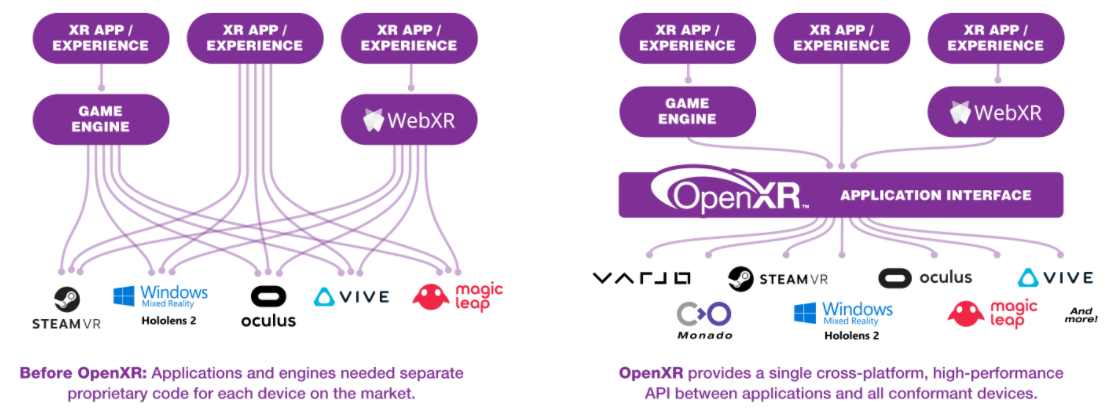
\includegraphics[width=0.9\textwidth]{oxr.png}
\caption{OpenXR vs OpenVR (Khronos Group)}
\end{figure}

Sul fronte grafico, mentre i motori commerciali (Unity, Unreal) o quelli proprietari, gestiscono le complesse API
grafiche internamente, per lo sviluppo nativo ed educativo, \texttt{WebGPU} si sta affermando come soluzione più
promettente.

Tuttavia, esiste attualmente un vuoto tecnologico per quanto riguarda l'API del \texttt{W3C} e \texttt{OpenXR}; tra
le due tecnologie non esiste alcun Graphic Binding ufficiale da parte di Khronos. Quest'ultimo infatti definisce
binding per \texttt{OpenGL}, \texttt{Vulkan}, \texttt{Direct3D} e \texttt{Metal}, ma non per \texttt{WebGPU}, essendo
quest'ultima un'RHI e non consistente in un driver nativo.

Il presente lavoro si inserisce esattamente in questo contesto; l'obbiettivo tecnico e scientifico è di dimostrare la
fattibilità di un layer di interoperabilità che permetta di implementare nativamente con \texttt{wgpu\_native} e che
questa implementazione possa comunicare con la complessa swapchain ed il frame-pacing di \texttt{OpenXR}.
Ciò permetterebbe di pensionare lo stack legacy e sostituirlo con uno all'avanguardia per il corso, con completa 
sostenibilità didattica e cross-platform per integrare i calcolatori di ogni studente.

\chapter{Design e implementazione}

Questo capitolo descrive in dettaglio la fase di implementazione del motore di rendering, che funge da \textit{Proof of
concept} per determinare la fattibilità dell'architettura sotto esame.
L'implementazione viene affrontata in modo incrementale, data la mancanza di esperienza per quanto riguarda le
tecnologie in questione, e viene divisa in tre pilastri fondamentali, che verranno esplorati nelle sezioni seguenti:

\begin{enumerate}
    \item Il motore grafico di base \texttt{WebGPU}, consistente nella costruzione di una pipeline di rendering 
        esplicita ed autonoma, utilizzando l'API \texttt{wgpu\_native}. Questa fase risolve le critiche relative
        all'allineamento della memoria, alla gestione esplicita dello stato ed al caricamento degli assets.
    \item L'integrazione di \texttt{OpenXR}, che vede l'implementazione di un'interfaccia indipendente dall'hardware
        per comunicare con i visori di realtà virtuale, gestendo il tracciamento spaziale, gli stati della sessione e
        l'acquisizione della swapchain.
    \item Il ciclo applicativo principale che fa da ponte tra i due sottosistemi, sincronizzando il rendering
        stereoscopico di \texttt{WebGPU} con i requisiti temporali di visualizzazione del compositor \texttt{OpenXR}.
\end{enumerate}

Analizzando queste tre fasi, questo capitolo illustra come i requisti ingegneristici teorici vengono tradotti in un
prototipo funzionale, ottimizzato e possibilmente multipiattaforma.

\newpage

\section{\texttt{WebGPU}}

La seguente sezione si concentra sulle funzionalità di \texttt{WebGPU} implementate, utili a raggiungere lo stesso
risultato dimostrato nel tutorial ufficiale del corso di realtà virtuale.

È importante che la codebase, sebbene facente uso di un'API con struttura e filosofia radicalmente differenti, sia
strutturata il più simile possibile a quella del corso, per rendere la comparazione il più semplice ed efficiente
possibile.

Altresì importante è tenere a mente che il codice prodotto è pensato per uno studente, è quindi da
considerare le piattaforme e il livello di confidenza nell'apprendere un'API del genere.

\subsection{Architettura}

A differenza di \texttt{OpenGL}, il quale mantiene uno stato globale e gestisce la sincronizzazione della memoria in
background, la nuova architettura richiede definizioni esplicite per ogni singola fase della pipeline. Per mantenere
una minima leggibilità e separare qualche responsabilità, pur lasciando la struttura simile a quella del tutorial del
corso per facilitarne la comparazione; per questo, seguendo l'architettura di corso, sono state modularizzate le classi:

\begin{itemize}
    \item \textbf{\texttt{Shader}}: Gestisce il caricamento, la compilazione ed il ciclo di vita degli Shader Modules
        WebGPU, partendo dalla sorgente di codice, nel linguaggio \texttt{WGSL} (Web GPU Shading Language).
        Evita il caricamento di file esterni direttamente dal punto d'entrata del motore.
        \begin{figure}[h]
        \centering
        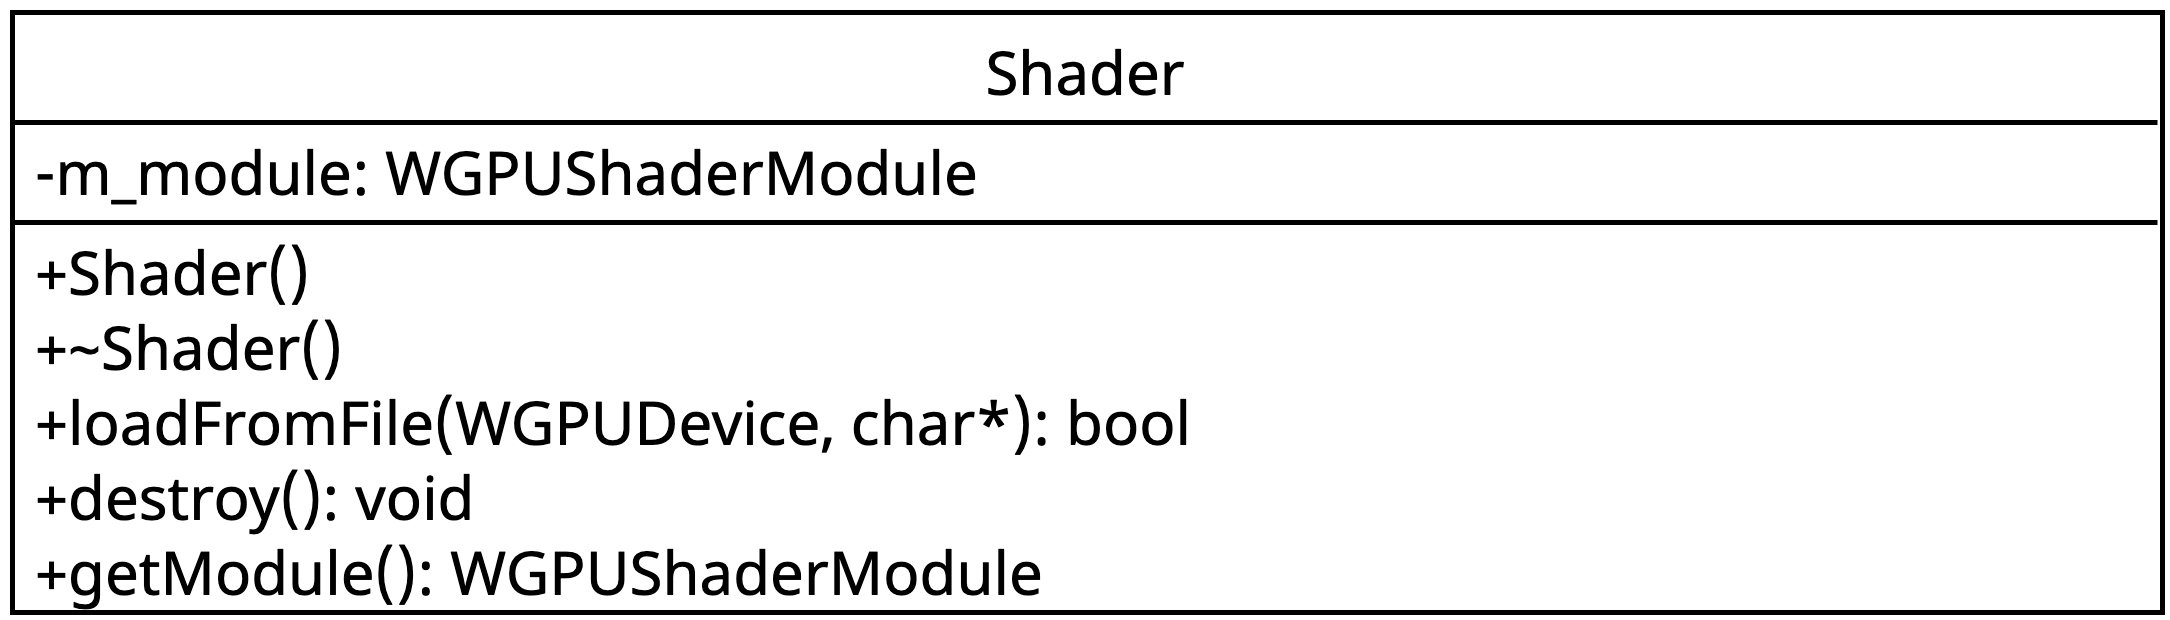
\includegraphics[width=0.7\textwidth]{shader_class.png}
        \caption{\texttt{Shader} class}
    \end{figure}
    \item \textbf{\texttt{WgpuBuffer}}: Incapsula la creazione e l'aggiornamento dei buffer GPU, detti
        \texttt{WGPUBuffer}, imponendo il rigoroso allineamento della memoria a 4 byte, richiesto dalle specifiche
        dell'API per i vertici ed i dati \textit{uniform}.
    \begin{figure}[h]
        \centering
        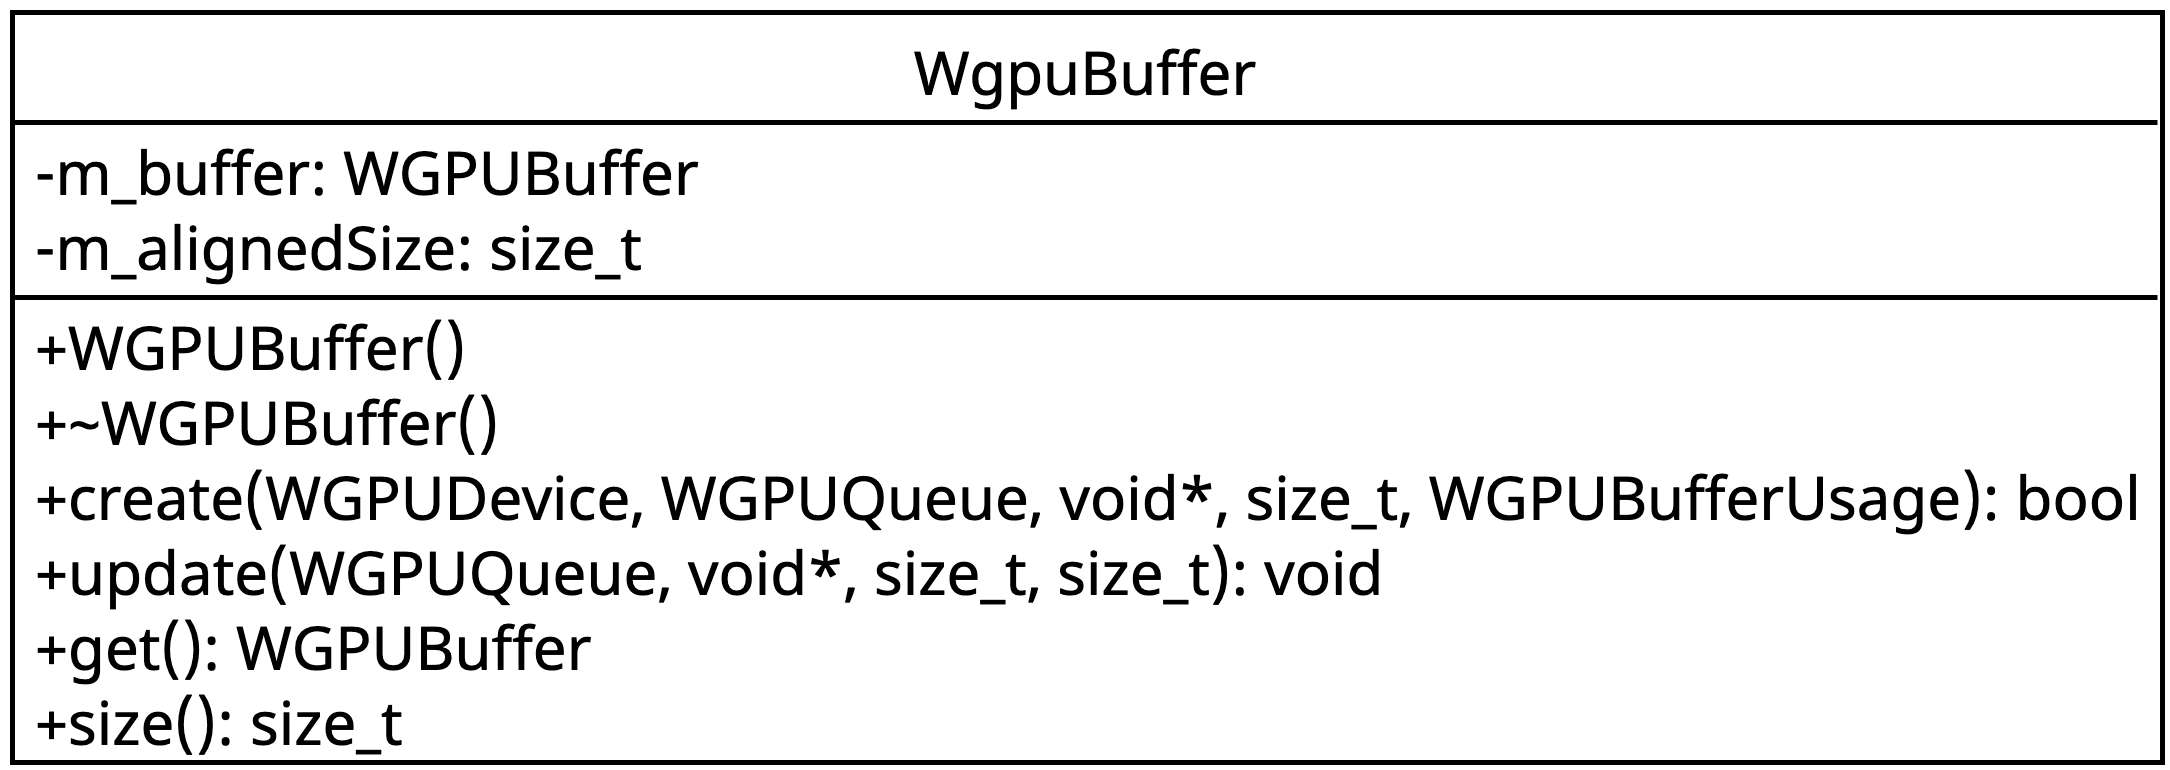
\includegraphics[width=0.7\textwidth]{wgpubuffer_class.png}
        \caption{\texttt{WgpuBuffer} class}
        \end{figure}
\end{itemize}

Questo incapsulamento garantisce che il ciclo principale dell'applicazione, includendo i descrittori della pipeline e la
codifica dei comandi, rimanga pulito e focalizzato esclusivamente sull'inizializzazione e l'orchestrazione.

\subsection{Inizializzazione contesto \& Windowing System}

La fase di inizializzazione del contesto, richiede il collegamento dell'istanza WebGPU ad un sistema di windowing al
livello del sistema operativo.
Questo requisito risulta relativamente complesso per l'integrazione della nuova API, in quanto questa è pensata per il
web, quindi non avendo alcun accesso diretto alle API di sistema per l'acquisizione della finestra.

\subsubsection{Windows}

Per i sistemi operativi della famiglia Windows, l'integrazione risulta relativamente lineare, grazie all'accesso diretto
alle API \texttt{Win32} fornite dalla libreria \texttt{GLFW}. Il descrittore specifico per questa piattaforma,
\texttt{WGPUSurfaceSourceWindowsHWND}, richiede la provvigione di due parametri fondamentali: l'handle dell'istanza
dell'applicazione (\texttt{hinstance}), recuperabile tramite la chiamata di sistema \texttt{GetModuleHandle}, e l'handle
della finestra nativa \texttt{hwnd}.
Come mostrato nel listing \ref{listing:winwinctx}, questi dati vengono incapsulati e concatenati direttamente al
descrittore generico della \textit{Surface}, sfruttando il meccansimo del puntatore \texttt{\gls{nextInChain}}.

\begin{listing}[!ht]
\begin{minted}{cpp}
WGPUSurfaceDescriptor surfaceDesc= {};
#if defined(_WIN32)
WGPUSurfaceSourceWindowsHWND hwndDesc = {
    .chain = { .sType = WGPUSType_SurfaceSourceWindowsHWND },
    .hinstance = GetModuleHandle(NULL),
    .hwnd = glfwGetWin32Window(window)
};
surfaceDesc.nextInChain = (WGPUChainedStruct*)&hwndDesc;
\end{minted}
\vspace{-0.75cm}
\caption{Inizializzazione contesto finestra (Windows)}
\label{listing:winwinctx}
\end{listing}
\vspace{-0.75cm}

\subsubsection{Linux}

Nel panorama Linux, l'acquisizione del contesto della finestra richiede un approccio dinamico a causa della coesistenza
di due differenti protocolli per server grafici: l'ormai legacy \textit{X11} ed il più moderno \textit{Wayland}. Per
garantire la massima portabilità e compatibilità, l'implementazione non assume a priori l'infrastruttura sottostante,
ma interroga la variabile d'ambiente \texttt{XDG\_SESSION\_TYPE} del sistema operativo per determinare il compositor
attualmente in uso.
A seconda del risultato (vedi listing \ref{listing:linwinctx}), l'algoritmo istanzia il descrittore appropriato
estraendo da \texttt{GLFW} i rispettivi puntatori nativi per il display e per la superficie di rendering.

\begin{listing}[!ht]
\begin{minted}{cpp}
#elif defined (__linux__)
char *envSession = std::getenv("XDG_SESSION_TYPE");
std::string windowingSystem = envSession ? envSession : "x11";
if (windowingSystem == "x11") {
    WGPUSurfaceSourceXlibWindow x11Desc = {
        .chain = { .sType = WGPUSType_SurfaceSourceXlibWindow },
        .display = glfwGetX11Display(),
        .window = glfwGetX11Window(window) };
    surfaceDesc.nextInChain = (WGPUChainedStruct*)&x11Desc;
} else if (windowingSystem == "wayland") {
    WGPUSurfaceSourceWaylandSurface waylandDesc = {
        .chain = { .sType = WGPUSType_SurfaceSourceWaylandSurface },
        .display = glfwGetWaylandDisplay(),
        .surface = glfwGetWaylandWindow(window) };
    surfaceDesc.nextInChain = (WGPUChainedStruct*)&waylandDesc;
}
\end{minted}
\vspace{-0.75cm}
\caption{Inizializzazione contesto finestra (Linux Wayland/X11)}
\label{listing:linwinctx}
\end{listing}
\vspace{-0.75cm}

\newpage

\subsubsection{macOS}

L'ecosistema Apple presenta il livello di complessità più alto per quanto riguarda la creazione della superficie,
poiché su queste piattaforme \texttt{WebGPU} si appoggia nativamente al backend grafico \texttt{Metal}.
Per evitare di dover introdurre nella codebase \texttt{C++} delle sorgenti scritte in \texttt{ObjectiveC}, che
richiederebbe l'uso di sorgenti \texttt{.mm}, l'implementazione sfrutta l'iniezione a runtime tramite la funzione
\texttt{objc\_msgSend} che permette di interagire direttamente con le librerie di sistema \texttt{Cocoa}.
Il processo, consultabile nel listing \ref{listing:macwinctx}, si occupa di estrarre dapprima l'oggetto
\texttt{NSWindow}, ne recupera poi la vista principale \texttt{contentView} e vi aggancia dinamicamente un livello di
rendering dedicato, chiamato \texttt{CAMetalLayer}.
Inoltre, durante questa fase, viene esplicitamenet disabilitata la proprietà \texttt{displaySyncEnabled} del layer
Metal; questo è un passaggio fondamentale per aggirare la sincronizzazione verticale forzata in modo aggressivo dal
\textit{Window Server} di macOS, permettendo all'applicazione di sbloccare il framerate per una migliore profilazione
delle performance.
Il livello così configurato viene finalmente passato al descrittore \texttt{WGPUSurfaceSourceMetalLayer}.

\begin{listing}[!ht]
\begin{minted}{cpp}
#elif defined(__APPLE__)
#include <objc/message.h>
#include <objc/runtime.h>
id nsWindow = glfwGetCocoaWindow(window);
id nsView = ((id(*)(id, SEL))objc_msgSend)(nsWindow, 
    sel_registerName("contentView"));
id caMetalLayerClass = (id)objc_getClass("CAMetalLayer");
id metalLayer = ((id(*)(id, SEL))objc_msgSend)(caMetalLayerClass,
    sel_registerName("layer"));
((void(*)(id, SEL, bool))objc_msgSend)(nsView,
    sel_registerName("setWantsLayer:"), true);
((void(*)(id, SEL, id))objc_msgSend)(nsView,
    sel_registerName("setLayer:"), metalLayer);
((void(*)(id, SEL, bool))objc_msgSend)(metalLayer,
    sel_registerName("setDisplaySyncEnabled:"), false);
WGPUSurfaceSourceMetalLayer metalDesc = {
    .chain = { .sType = WGPUSType_SurfaceSourceMetalLayer },
    .layer = metalLayer
};
surfaceDesc.nextInChain = (WGPUChainedStruct*)&metalDesc;
#endif
\end{minted}
\vspace{-0.75cm}
\caption{Inizializzazione contesto finestra (macOS)}
\label{listing:macwinctx}
\end{listing}

Una volta configurato il descrittore specifico per la piattaforma host corrente tramite la catena di strutture
\texttt{\gls{nextInChain}}, la superficie viene concretamente istanziata e restituita al ciclo di vita dell'applicazione
tramite la chiamata nativa dell'API.

\begin{minted}{cpp}
return wgpuInstanceCreateSurface(instance, &surfaceDesc);
\end{minted}

\newpage

\subsection{Gestione Memoria e assets}

Il passaggio dal \texttt{glTexImage2D} di \texttt{OpenGL} al sistema adottato da \texttt{WebGPU} richiede il calcolo
manuale degli \textit{stride} di memoria. La libreria \texttt{stb\_image} è stata integrata per caricare gli assets
direttamente in un formato \textit{top-down}, corrisponendo nativamenta al sistema di coordinate delle texture
\texttt{WebGPU} ed eliminando la necessità di invertire l'asse $y$ durante il caricamento.

L'API impone un vincolo sui caricamenti delle texture tramite \texttt{wgpuQueueWriteTexture}: il parametro
\texttt{bytesPerRow} deve essere obbligatoriamente un multiplo di $256$ bytes. Questo problema è stato risolto
calcolando e applicando matematicamente un padding al buffer dei dati grezzi dell'immagine, prima di consegnarlo alla
GPU.

\begin{listing}[!ht]
\begin{minted}{cpp}
uint32_t bytesPerRow = (texWidth * 4 + 255) & ~255;
std::vector<uint8_t> paddedData(bytesPerRow * texHeight, 0)
for (int y = 0; y < texHeight; ++y) {
    memcpy(&paddedData[y*bytesPerRow], &rawData[y*texWidth*4], texWidth*4);
}
\end{minted}
\vspace{-0.75cm}
\caption{Generazione dei dati texture con padding}
\label{listing:texpad}
\end{listing}

Un altro fondamentale cambiamento di paradigma riguarda l'allineamento delle strutture tra \texttt{C++} e \texttt{WGSL}.
Questo infatti impone rigorose regole di layout nella memoria, nelle quali tipi di dati come \texttt{vec3} devono essere
strettamente allineati a limiti di $16$ bytes.
Per prevenire la desincronizzazione della memoria tra le \texttt{struct} di \texttt{C++} a $128$ bytes e la
\texttt{struct WGSL} attesa, da $144$ bytes, è stato introdotto un padding manuale nelle strutture dati \texttt{C++} per
soddisfare le aspettative di memoria della GPU, senza sprecare larghezza di banda.

\begin{listing}[!ht]
\begin{minted}[highlightlines={10}]{cpp}
struct LightMaterialUniforms {
    glm::vec4 lightPosition;
    glm::vec4 lightAmbient;
    glm::vec4 lightDiffuse;
    glm::vec4 lightSpecular;
    glm::vec4 matAmbient;
    glm::vec4 matDiffuse;
    glm::vec4 matSpecular;
    float matShininess;
    float padding[3];
};
\end{minted}
\vspace{-0.75cm}
\caption{Esempio di allineamento a $16$ bytes}
\label{listing:wgslpad}
\end{listing}

\subsection{Pipeline e Bind Group}

La pipeline di rendering funge da oggetto di stato immutabile. Il prototipo utilizza un modello di illuminazione
\textit{Blinn-Phong}, proprio come nel tutorial del corso, il tutto tradotto in una \textit{Shader} scritta nel
linguaggio \texttt{WGSL}. Durante la creazione della pipeline, viene sfruttata la funzionalità di \textit{Auto-Layout}.

\begin{minted}{cpp}
pipelineDesc.layout = nullptr;
\end{minted}

Questo istruisce il backend WebGPU a inferire dinamicamente il layout del Bind Group, direttamente dalle annotazioni
del linguaggio di shading (\texttt{@group} e \texttt{@binding}), riducento significativamente la verbosità del
\texttt{C++}.

Le risorse da fornire al programma shader sono divise in due distinti Bind Group in base alla loro frequenza di
aggiornamento:

\begin{enumerate}
    \item \textbf{Bind Group 0}: contiene gli Uniform Buffer per le matrici \textit{Model-View-Projection} ed i
        parametri dei materiali di illuminazione, aggiornati ad ogni frame
    \item \textbf{Bind Group 1}: contiene il \textit{Sampler} e la \textit{Texture View}, che rimangono statici per
        tutto il ciclo di vita dell'applicazione
\end{enumerate}

Inoltre, le rigide regole di validazione dell'API hanno richiesto una gestione esplicita delle \textit{C Strings}.
Con i recenti aggiornamenti delle API, gli entrypoint degli shader devono essere passati come oggetti di tipo
\texttt{WGPUStringView}, che abbinano il contenuto della stringa con una macro di lunghezza specifica
(\texttt{WGPU\_STRLEN}), piuttosto che come puntatori terminati da carattere nullo, al fine di gestire la sicurezza
della memoria attraverso i confini del backend Rust.

\subsection{Command Encoder e Render Loop}

Il ciclo principale vede un \texttt{WGPUCommandEncoder} che registra una serie di istruzioni all'interno di un command
buffer, che viene successivamente sottomesso alla queue della GPU in una singola operazione.

Una cruciale implementazione di stabilità all'interno del ciclo di rendering è la gestione dello stato di acquisizione
della \texttt{WGPUSurfaceTexture}. Le latenze del sistema operativo, come il ridimensionamento o la riduzione ad icona
della finestra potrebbero far sì che la superficie "perda" temporaneamente accesso alla texture del frame corrente;
l'aggiunta di una \textit{guard clause} che valuti lo stato \texttt{WGPUSurfaceGetCurrentTextureStatus\_Success}
impedisce al backend Rust di andare in \textit{panic} alla ricezione di un puntatore nullo, garantendo la totale
robustezza del motore in caso di eventi esterni.

Infine, il \texttt{WGPURenderPassDescription} richiede definizioni esplicite e complete, inclusa la specifica del
parametro \texttt{depthSlice} a \texttt{WGPU\_DEPTH\_SLICE\_UNDEFINED}, per i color attachment 2D, una configurazione
necessaria per conformarsi in modo rigoroso alle specifiche di rendering delle texture 3D, recentemente introdotte
in WebGPU.

\newpage

\section{Interoperabilità \texttt{WebGPU-OpenXR}}

L'integrazione tra \texttt{WebGPU} e \texttt{OpenXR} presenta una sfida architetturale fondamentale legata ai paradigmi
di sicurezza ed astrazione delle due API; \texttt{WebGPU}, per sua natura, è agnostica e sicura: il suo obbiettivo è
di nascondere completamente i dettagli hardware sottostanti dietro ad un'interfaccia unificata. Al contrario,
\texttt{OpenXR} per operare in ambiente VR richiede un'accesso esplicito e diretto ai puntatori nativi della GPU, ed
alle allocazioni di memoria delle immagini per poter gestire la swapchain a bassa latenza.

Nella versione più recente\footnote{\url{https://github.com/gfx-rs/wgpu-native/tree/v29.0.0.0}}, le funzioni di
estrazione per il backend \texttt{Vulkan} sono state rimosse dall'API pubblica, sigillando di fatto i puntatori nativi
all'interno dell'Hardware Abstraction Layer, scritto in Rust. Ciò rende impossibile l'inizializzazione standard di una
\texttt{XrSession} basata sul contesto grafico di WebGPU.

\chapter{Test e validazione}

\section{Risultati}

\chapter{Risultati}

\section{Manuale d'uso}

\chapter{Conclusioni}

\section{Sviluppi futuri}

\blankpage
\pagenumbering{Roman}
\printglossary[title=Glossario, toctitle=Glossario]

\blankpage
\printbibliography[heading=bibintoc, title=Sitografia]

\end{document}
